\subsection{Construction of Grid Extrusion}
\label{sec:construction_of_grid_extrusion}
Given a strip of size $w\times Y$, we will consider the evolution of the cross sections along the length $Y$.
Imagine that there are $T = \frac Y\epsilon$ time steps over which the cross section evolves along the $y$-axis.
Consider the decomposition of $Y$ as
$$Y = (1 + D_1) + (1 + D_2) + (1 + D_) +\cdots + (1 + D_{n-1})$$
Here, the times corresponding to
\begin{itemize}
	\item the $i^{th}$ ''1'' is realized as the strip $i-1\le y\le i$
	\item $D_i$ is the transition between $i-1\le y\le i$ and $i\le y\le i+1$
\end{itemize}

\subsection{Construction of Strip Extrusion}
\label{sec:construction_of_strip_extrusion}

\subsubsection{Level Shifting}
\label{sec:level_shifting}

\graphicspath{{./figures/level_shift/}}%
\begin{figure}[t!]%
    \centering
    \begingroup%
        \def\svgwidth{0.25\textwidth}
        \captionsetup[subfigure]{width=0.25\textwidth}
        \subfloat[Higher initial level. Top segment moves down.]{%
            \input{./figures/level_shift/column0.pdf_tex}
            \label{fig:level_shift0}
        }%
    \endgroup
    \subfloat[Two segments created. New segments are aligned with top segment, and move down. Vertical segments move inwards.] {%
        \def\svgwidth{0.24\textwidth}
        \input{./figures/level_shift/column1.pdf_tex}%
        \def\svgwidth{0.25\textwidth}
        \input{./figures/level_shift/column2.pdf_tex}%
        \label{fig:level_shift1}
    }%
    \def\svgwidth{0.25\textwidth}
    \subfloat[Two more segments created. Vertical segments reverse direction.] {%
        \input{./figures/level_shift/column3.pdf_tex}%
    %}%
        \def\svgwidth{0.27\textwidth}
    %\subfloat[] {
        \input{./figures/level_shift/column4.pdf_tex}%
    %}%
        \def\svgwidth{0.29\textwidth}
    %\subfloat[] {
        \input{./figures/level_shift/column5.pdf_tex}%
        \label{fig:level_shift2}
    }%

    \subfloat[Level shift completed with four new horizontal segments.] {%
        \def\svgwidth{0.29\textwidth}
        \input{./figures/level_shift/column6.pdf_tex}%
        \def\svgwidth{0.34\textwidth}
        \input{./figures/level_shift/column7.pdf_tex}%
        \label{fig:level_shift3}
    }%
    \begingroup
        \def\svgwidth{0.27\textwidth}
        \captionsetup[subfigure]{width=0.24\textwidth}
        \subfloat[Flat folded state.]{%
            \input{./figures/level_shift/column8.pdf_tex}%
            \label{fig:level_shift4}
        }%
    \endgroup%
    \caption{Level shifting gadget. The separation along the $Y$ direction illustrates the layering. The red line denotes the boundary of the cross section.}
    \label{fig:level_shift}
\end{figure}%


\subsection{Construction of Strip Connectors}
\label{sec:construction_of_strip_connectors}

\subsubsection{Alignment with Level Shifts}
\label{sec:alignment_with_level_shifts}

\begin{figure}[!htb]
\graphicspath{{figures/column_connector}}
    \centering
    \subfloat[Initial height.]{
        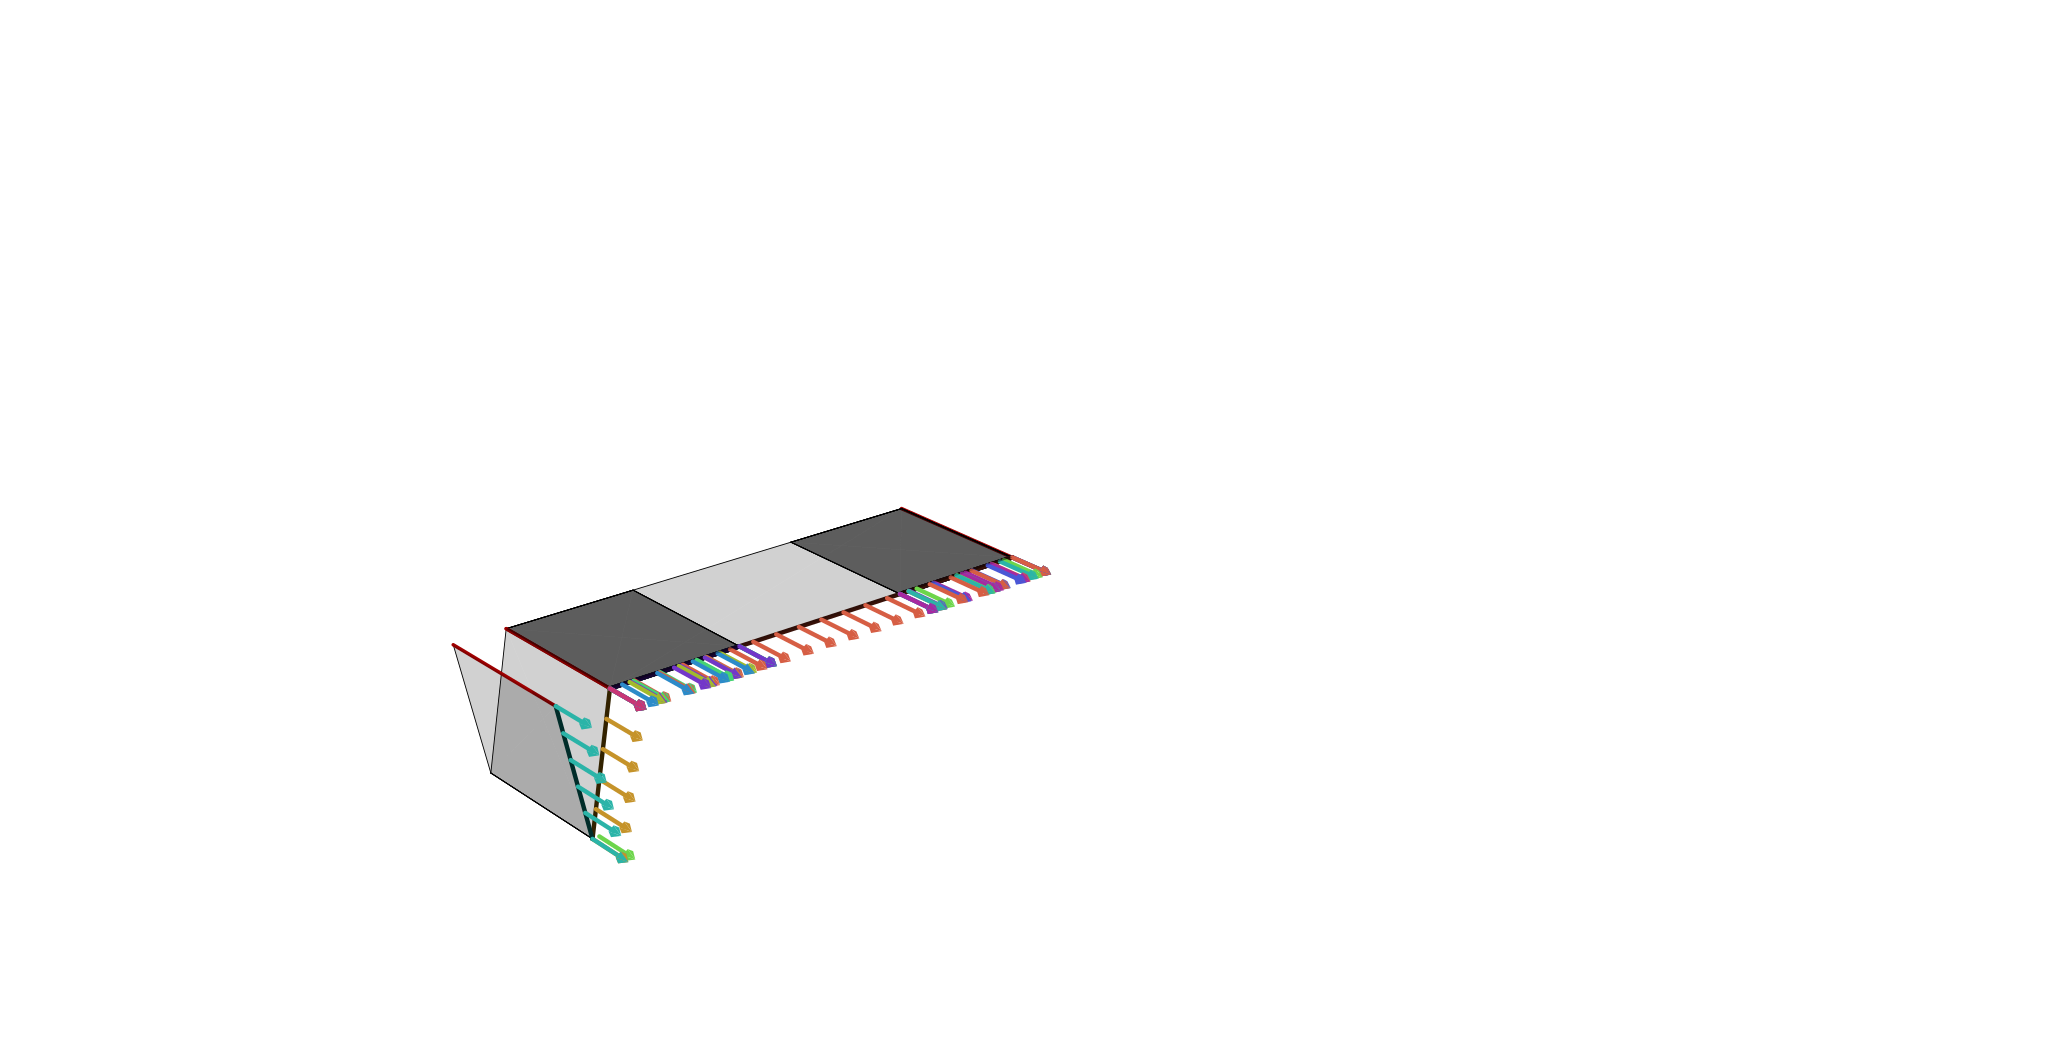
\includegraphics[width=0.23\textwidth]{figures/column_connector/column0.pdf}
    }%
    \subfloat[Connector moves outwards.]{
        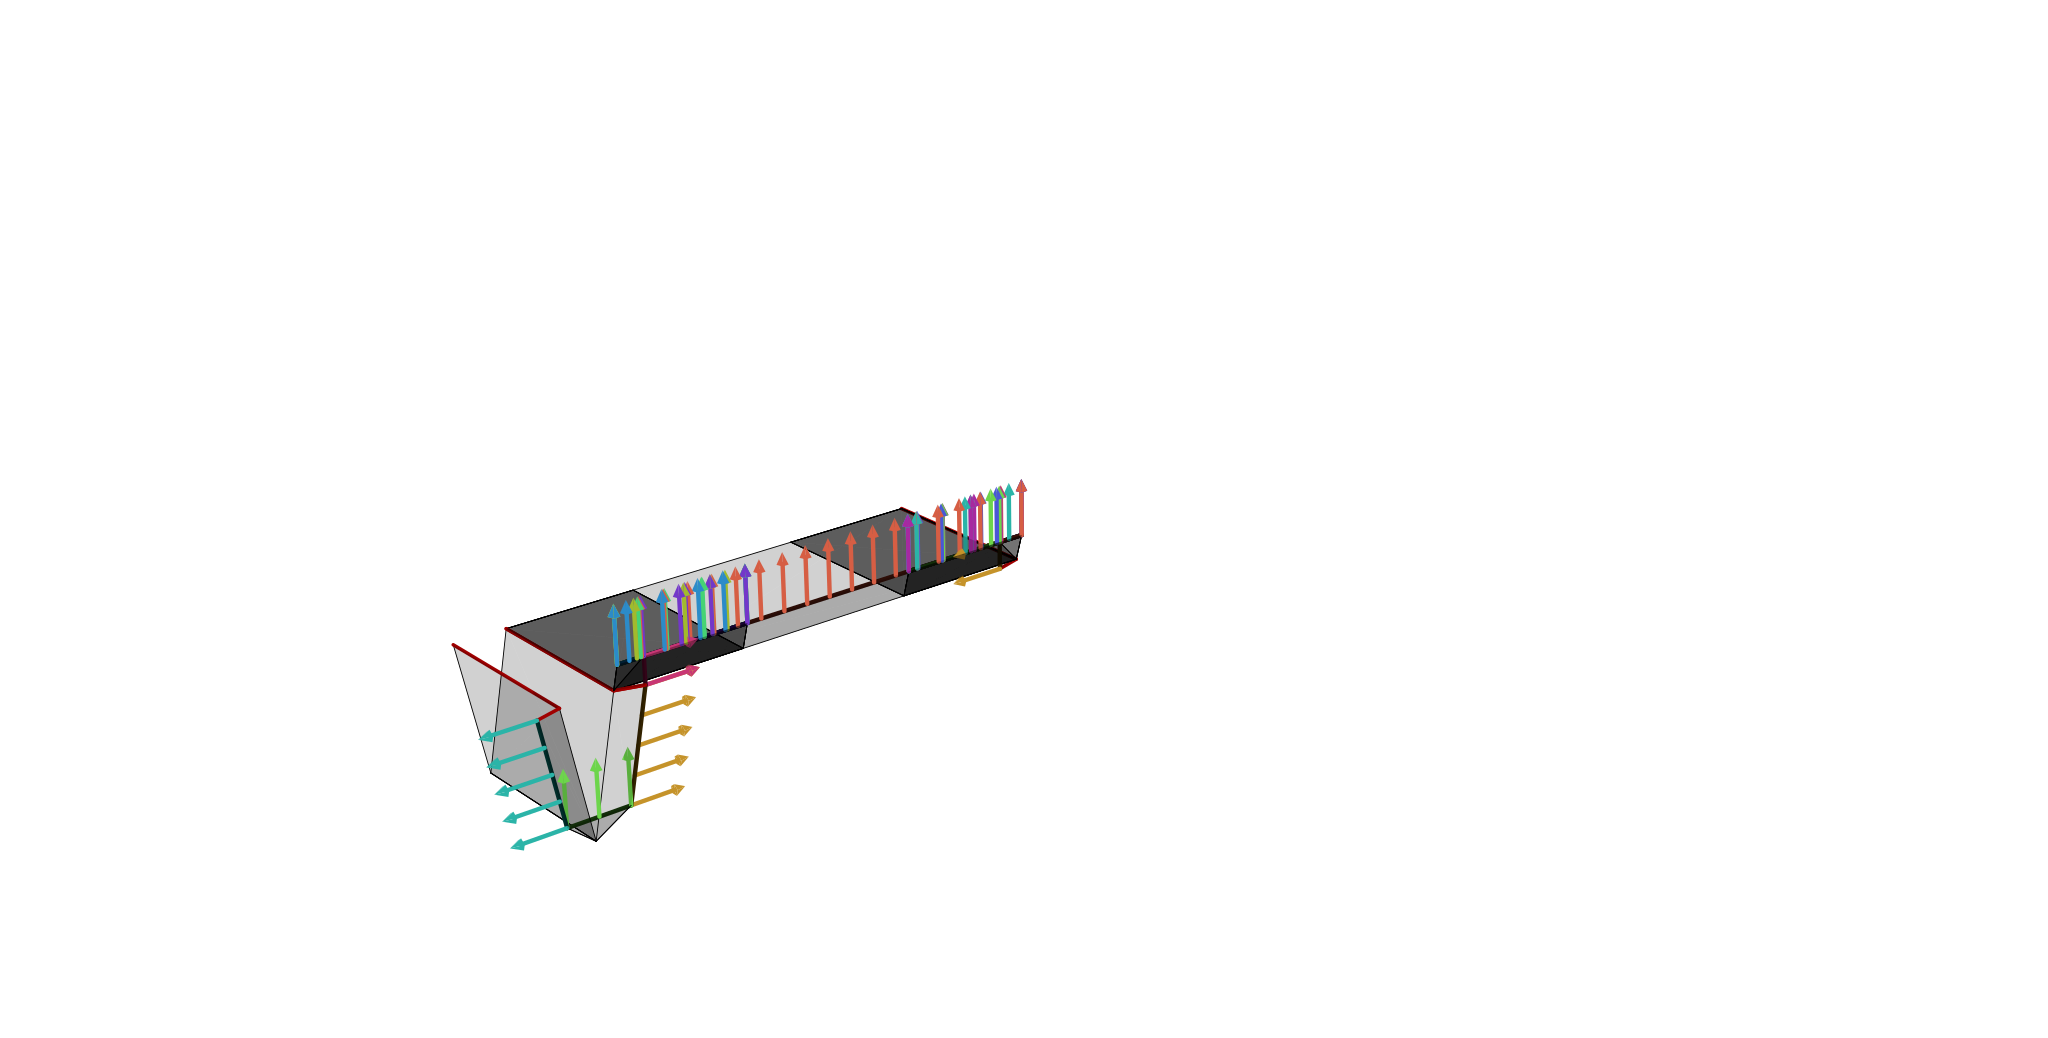
\includegraphics[width=0.21\textwidth]{figures/column_connector/column1.pdf}
    %}
    %\subfloat[]{
        
\includegraphics[width=0.21\textwidth]{figures/column_connector/column2.pdf}
    }%
    \subfloat[Connector at maximum width.]{
        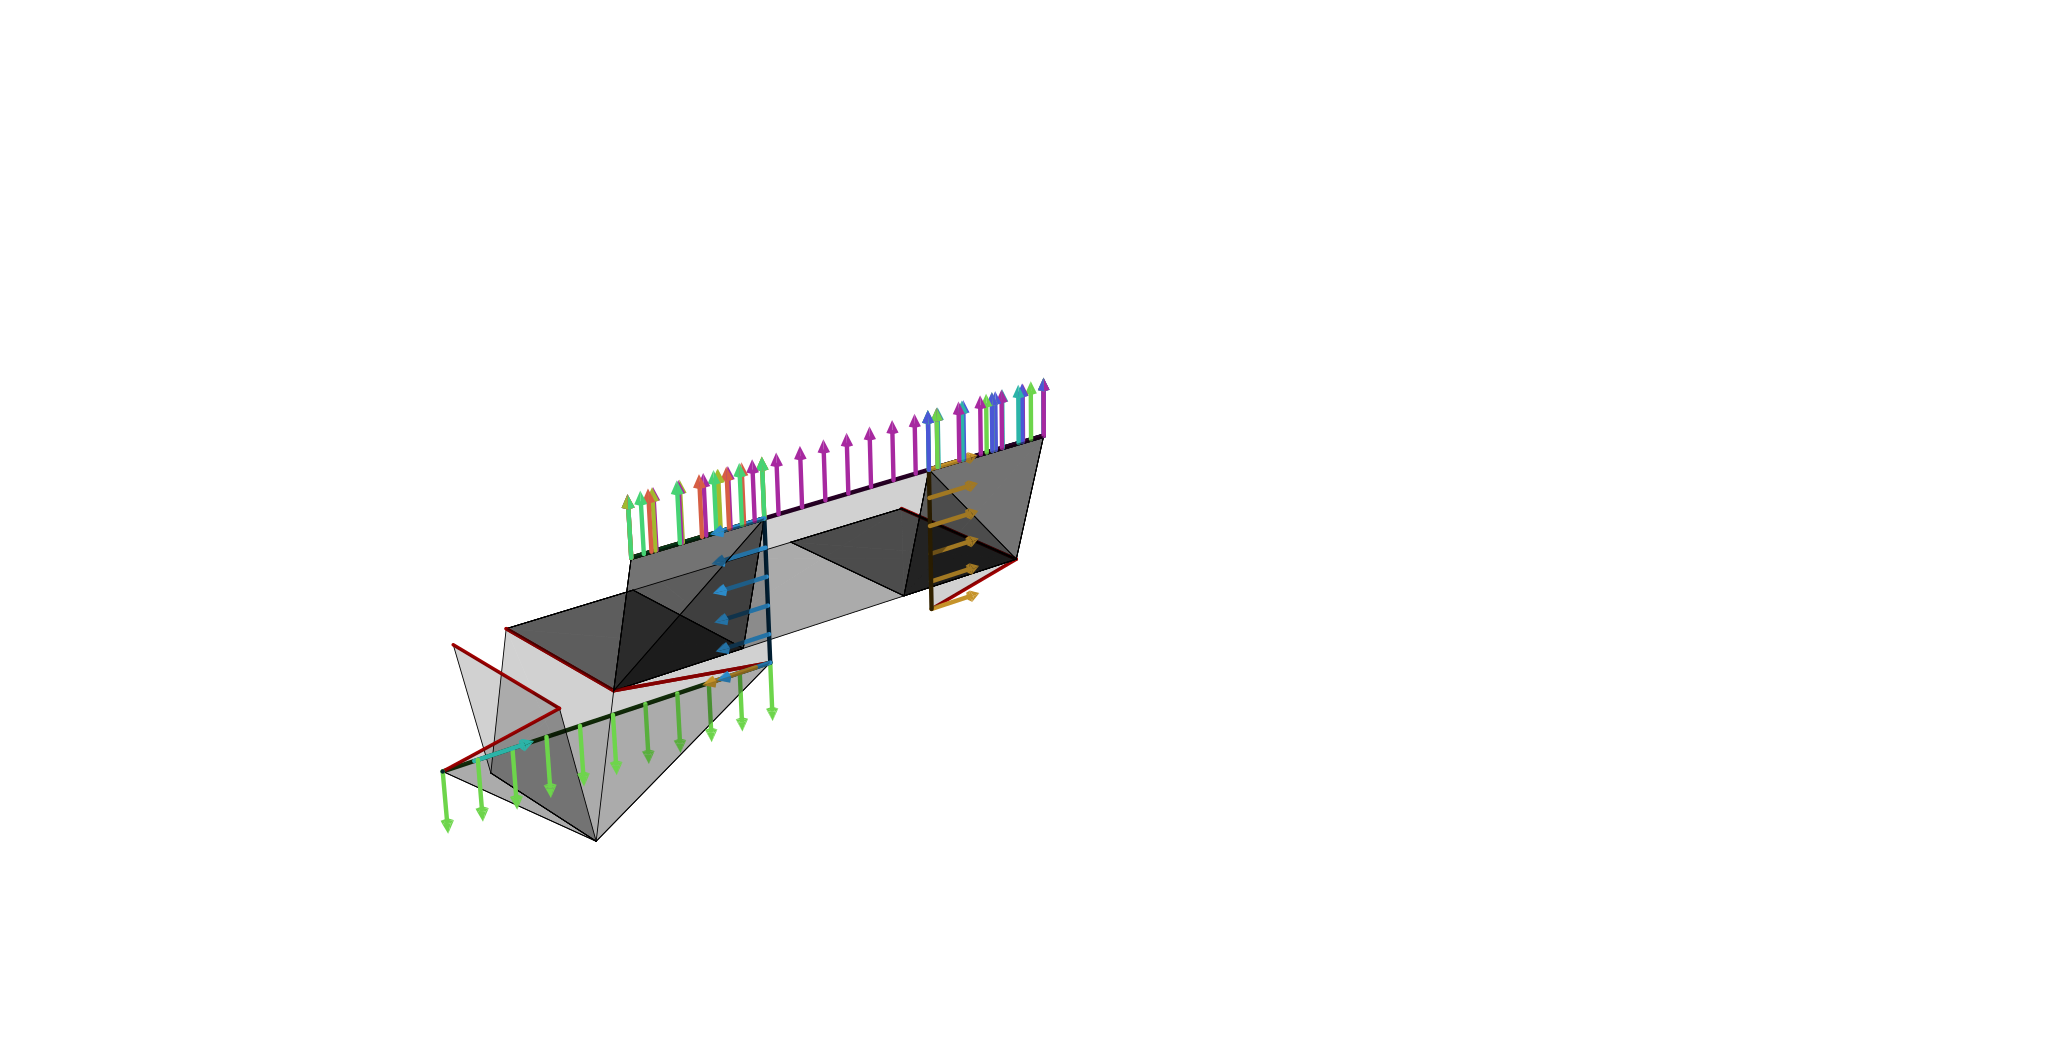
\includegraphics[width=0.24\textwidth]{figures/column_connector/column3.pdf}
    }%

    \subfloat[Connector moves inwards.]{
        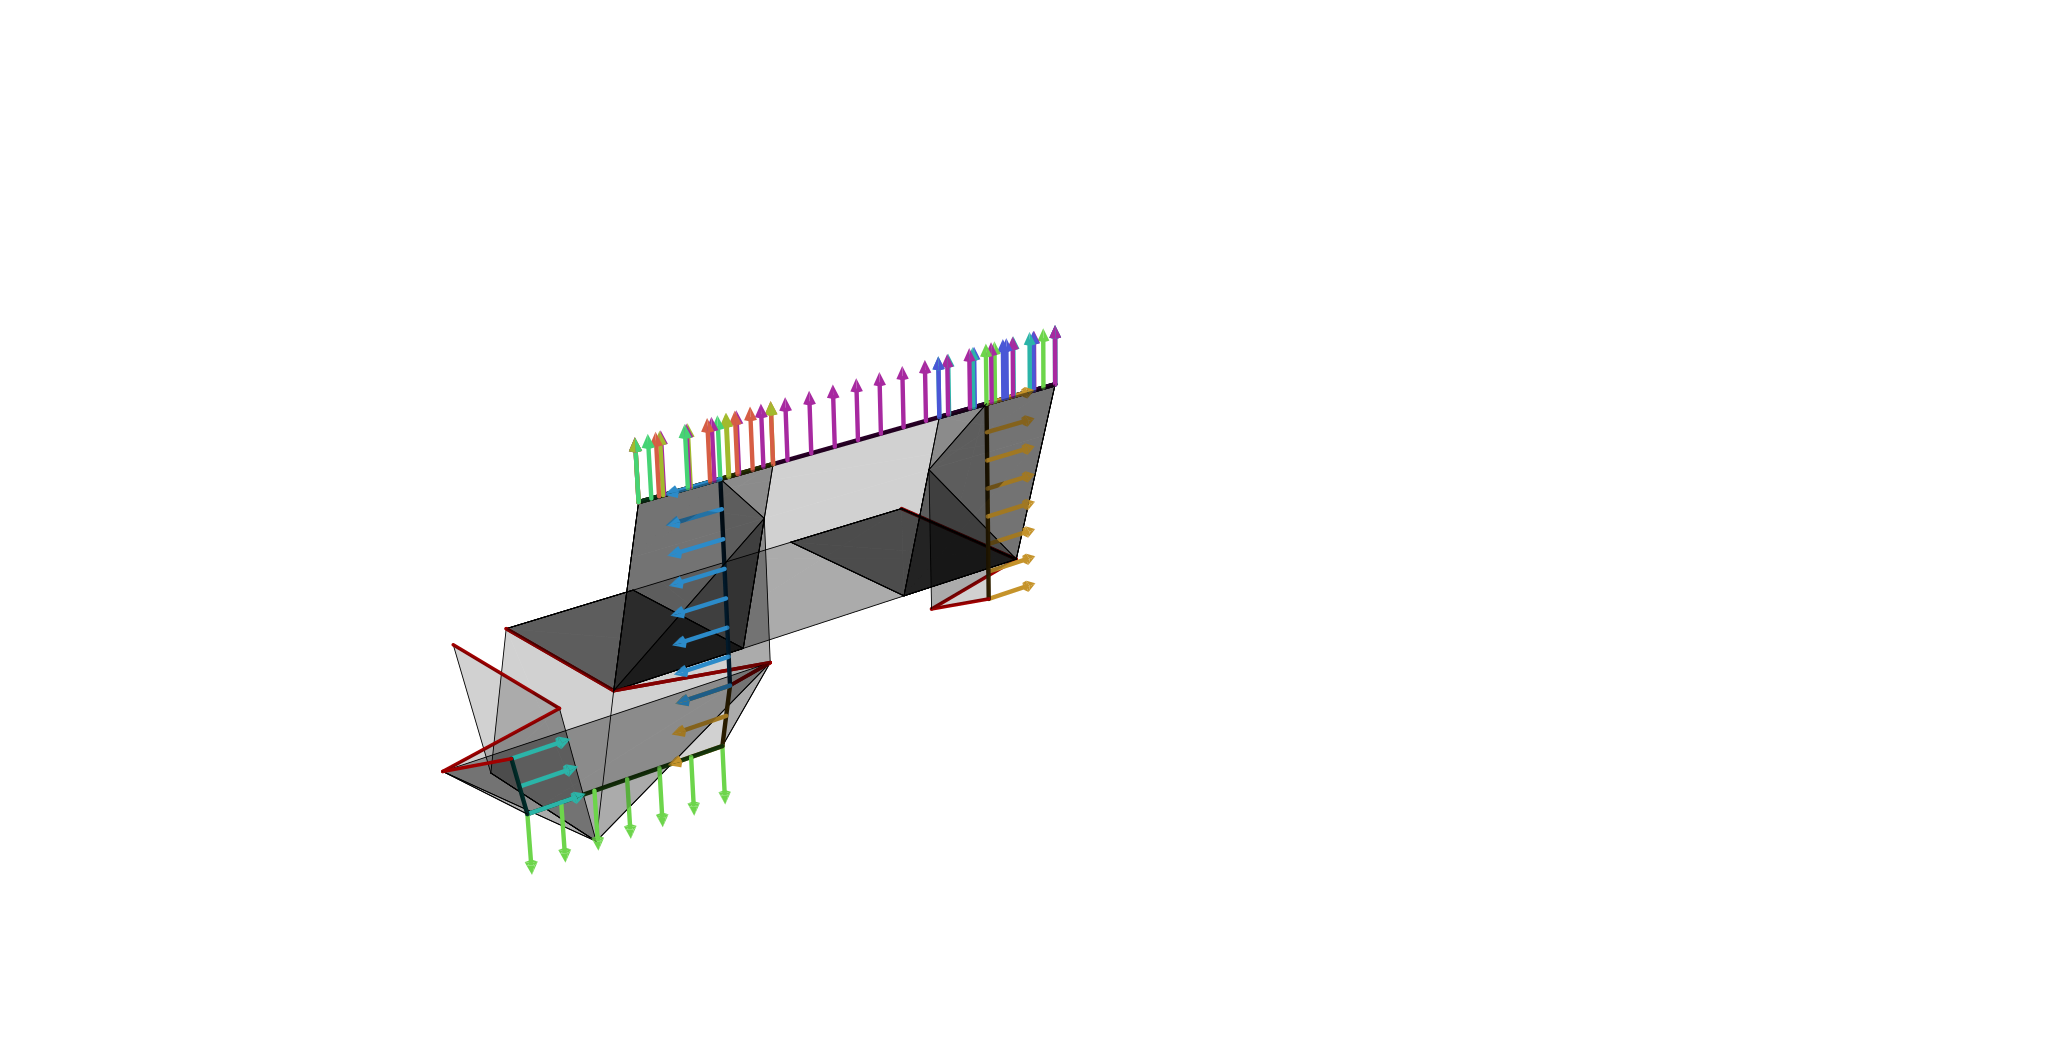
\includegraphics[width=0.23\textwidth]{figures/column_connector/column4.pdf}
    %}
    %\subfloat[]{
        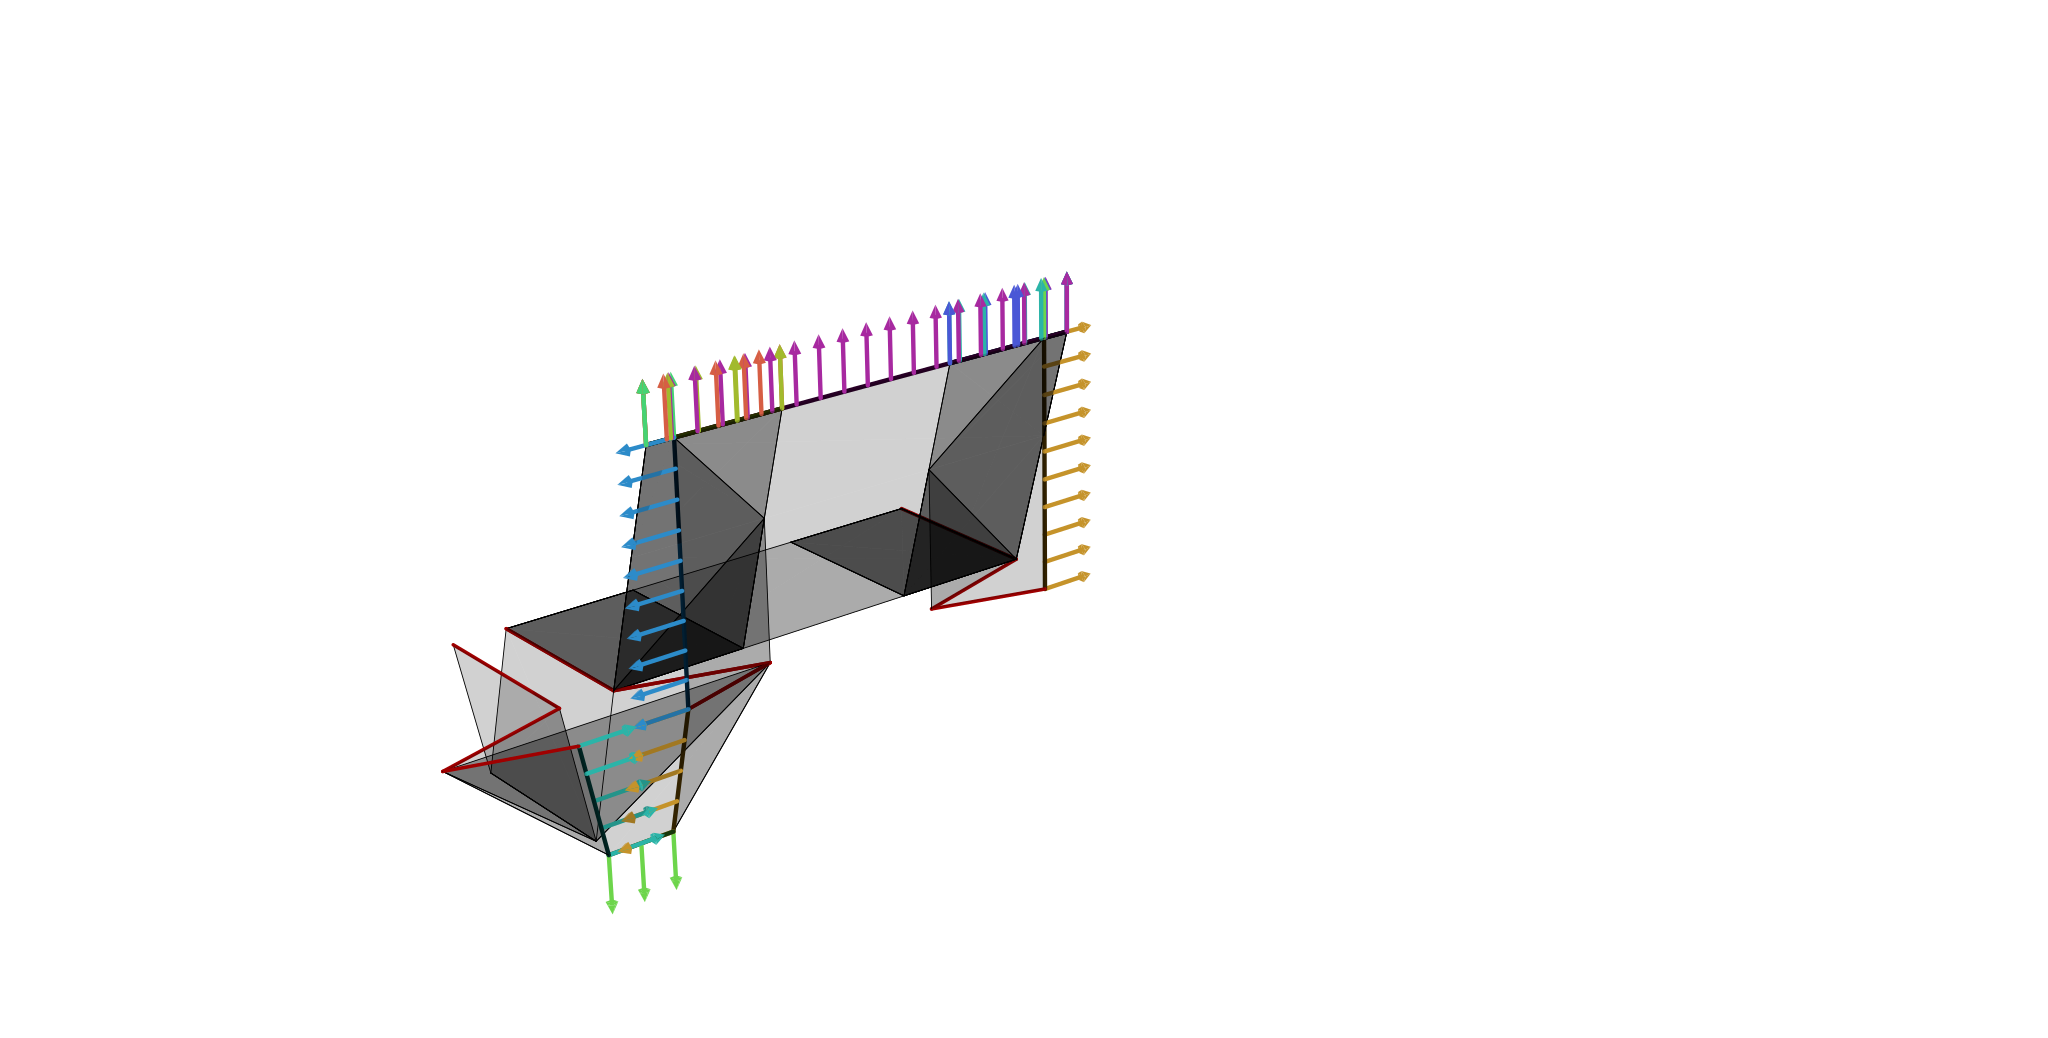
\includegraphics[width=0.23\textwidth]{figures/column_connector/column5.pdf}
    }%
    \subfloat[Back to \textbf{(a)}.]{
        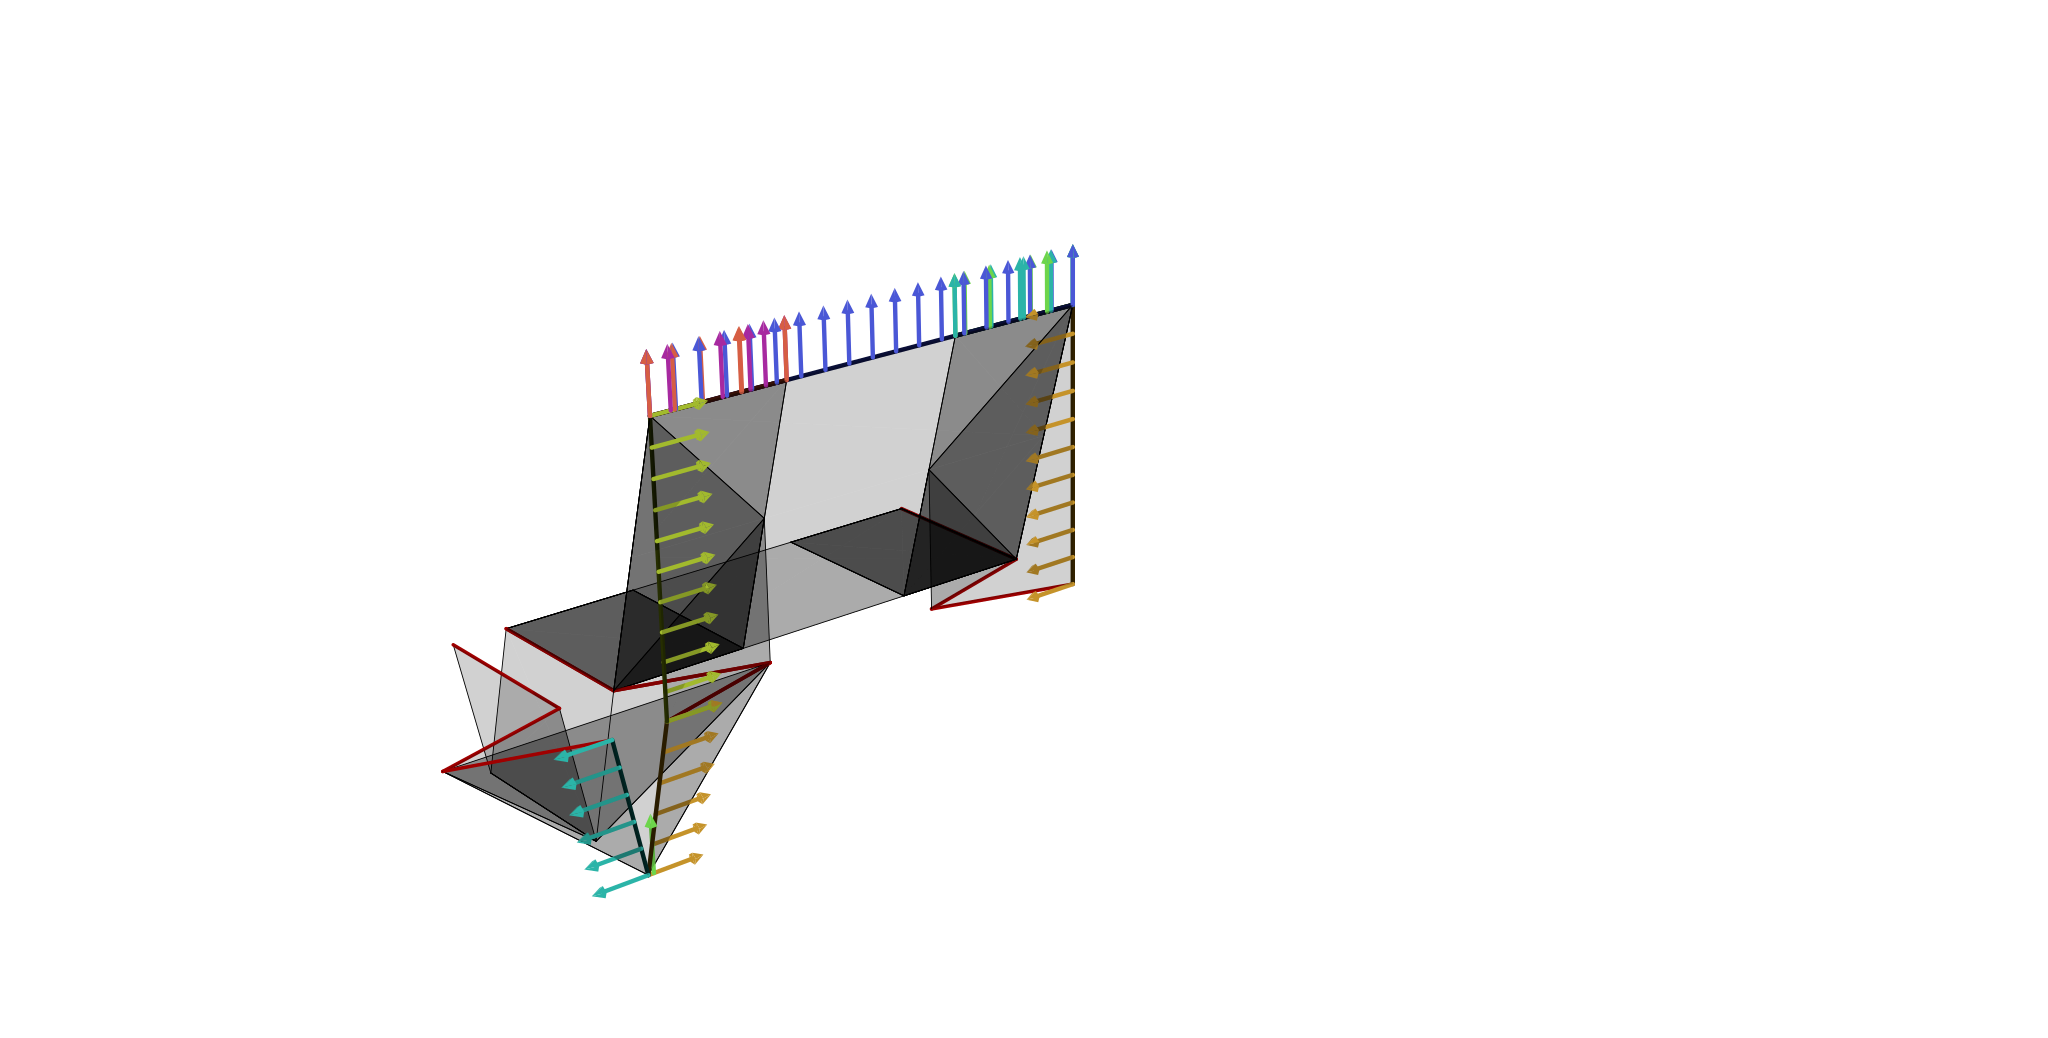
\includegraphics[width=0.23\textwidth]{figures/column_connector/column6.pdf}
    }%
    \subfloat[Same as \textbf{(b)}.]{
        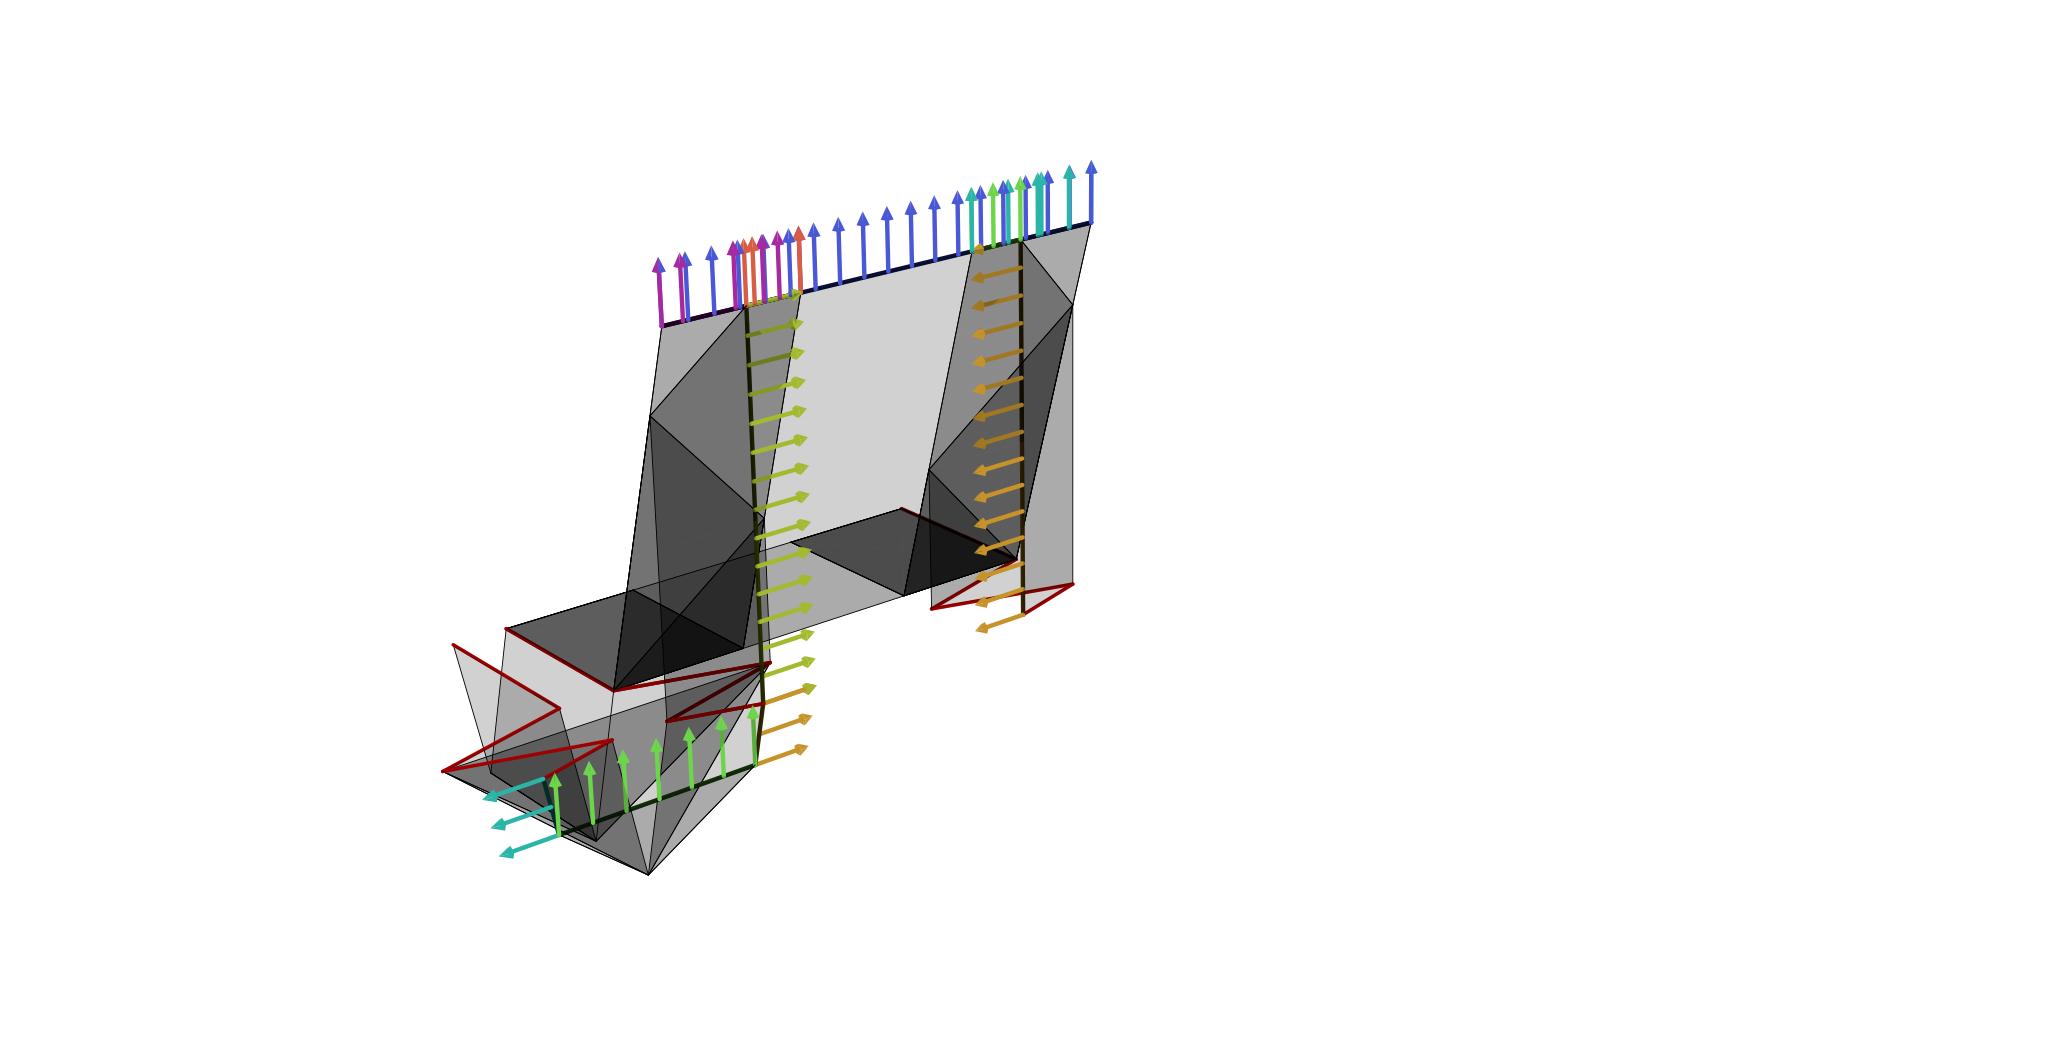
\includegraphics[width=0.23\textwidth]{figures/column_connector/column7.pdf}
    }%

    \subfloat[Same as \textbf{(d)}.]{
        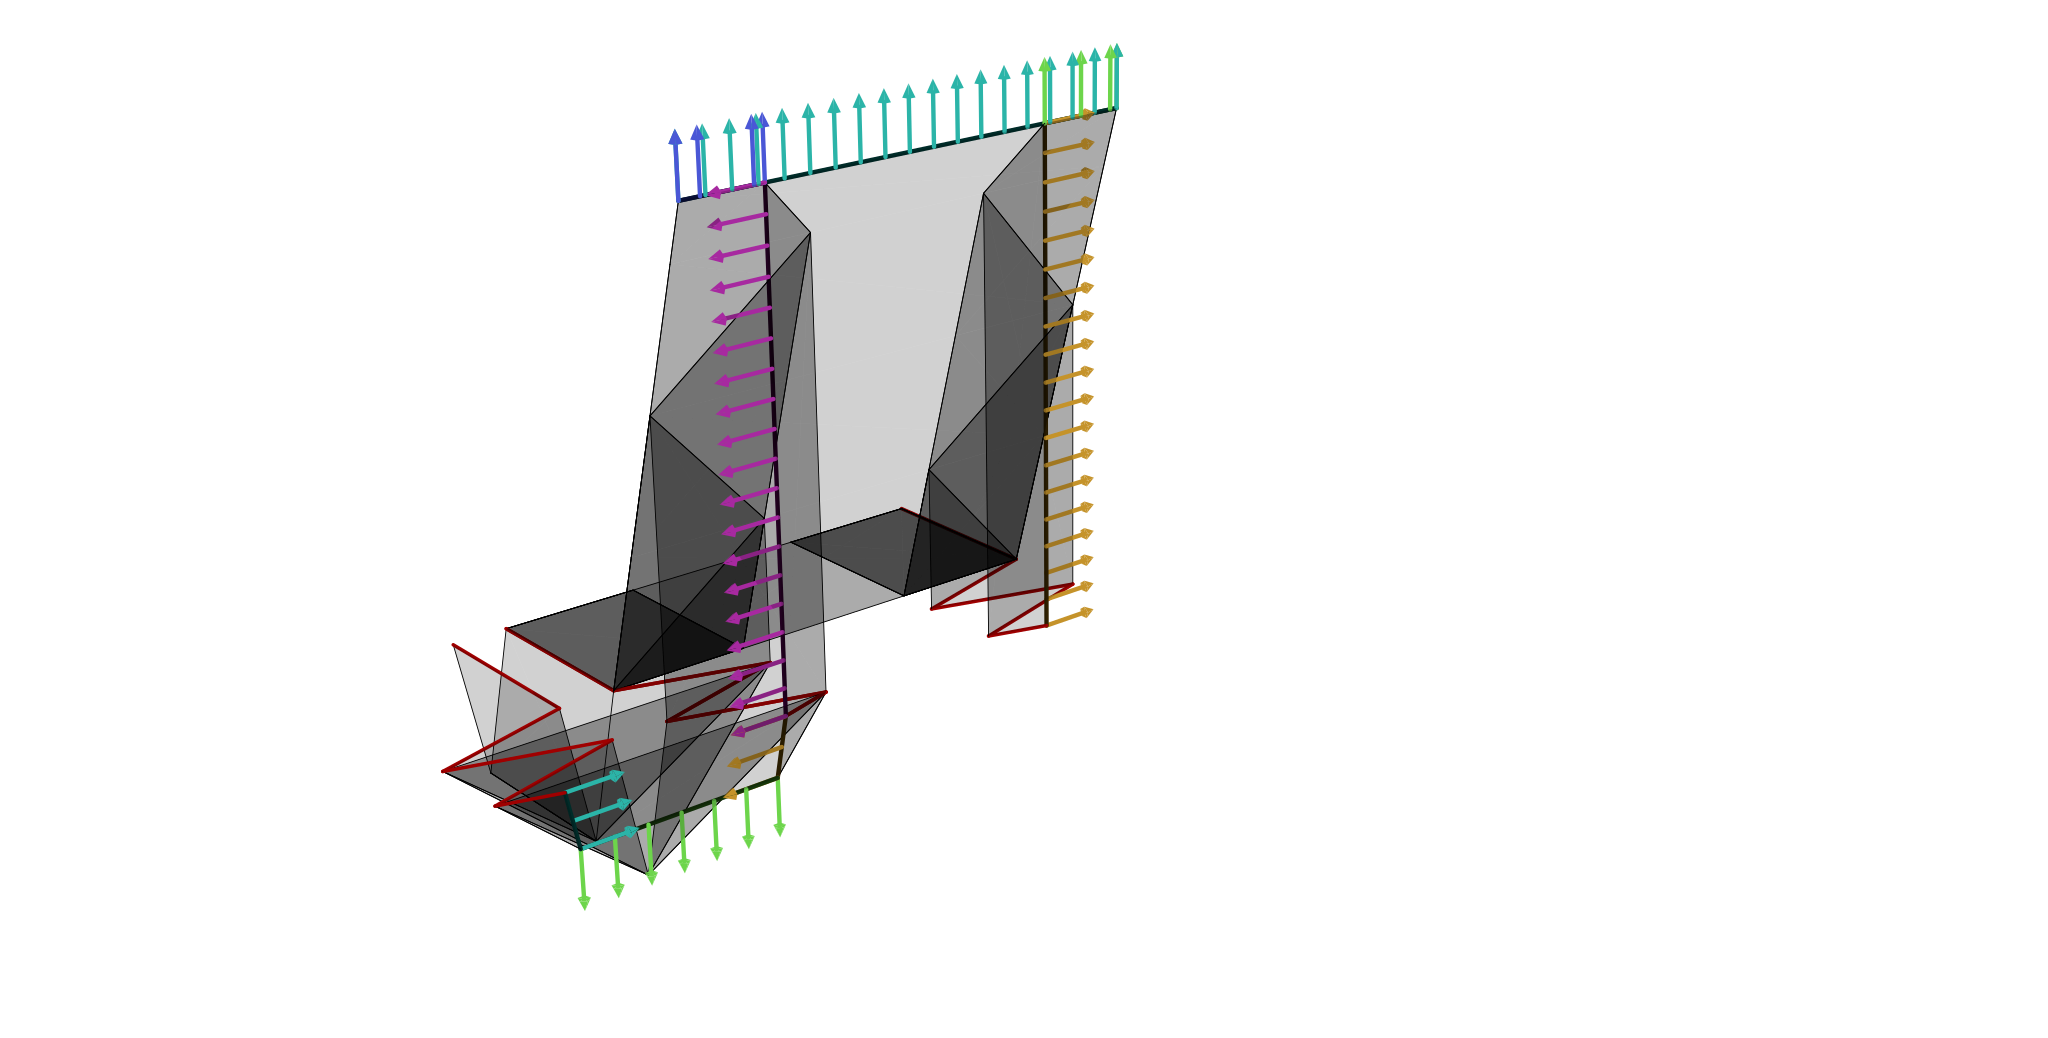
\includegraphics[width=0.29\textwidth]{figures/column_connector/column8.pdf}
    }%
    \subfloat[Level shift complete, and next level continues.]{
        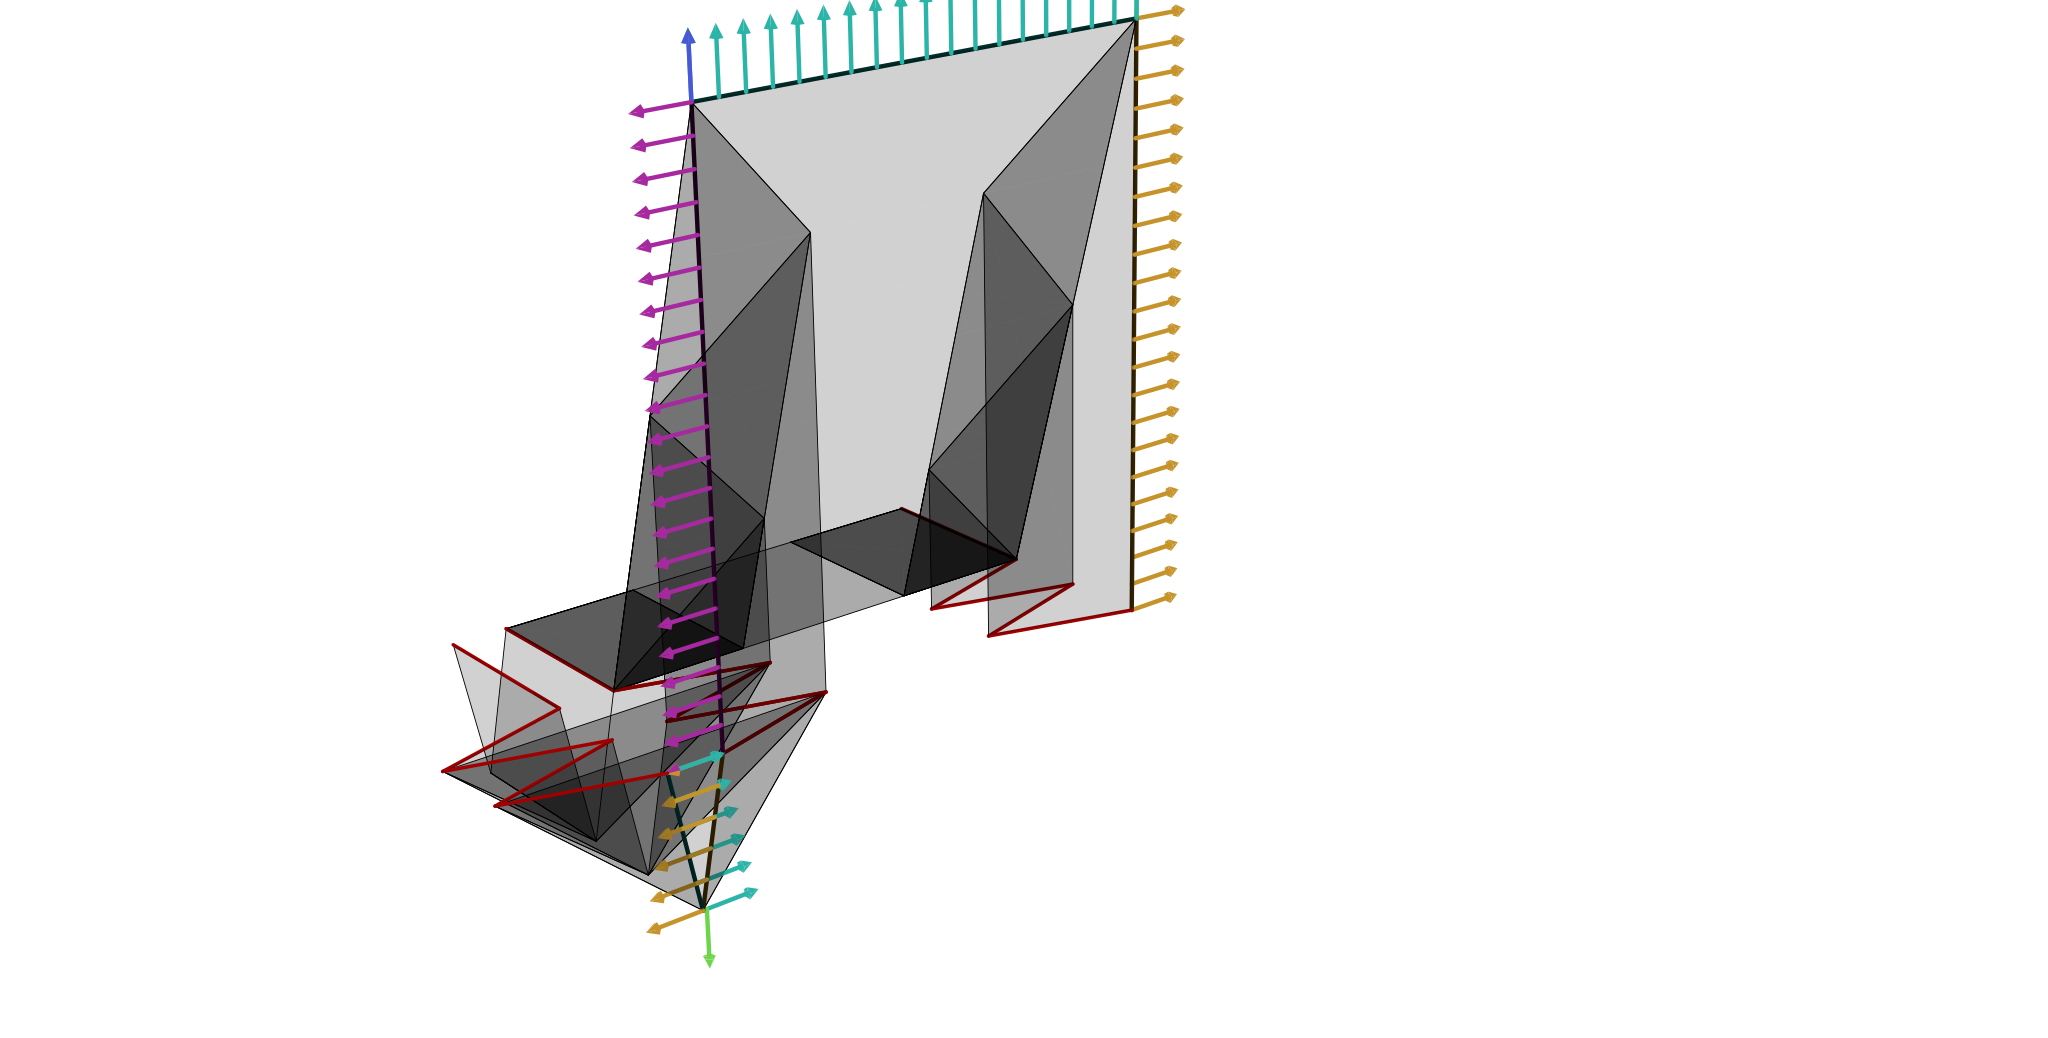
\includegraphics[width=0.29\textwidth]{figures/column_connector/column9.pdf}
    %}
    %\subfloat[Column and connector]{
        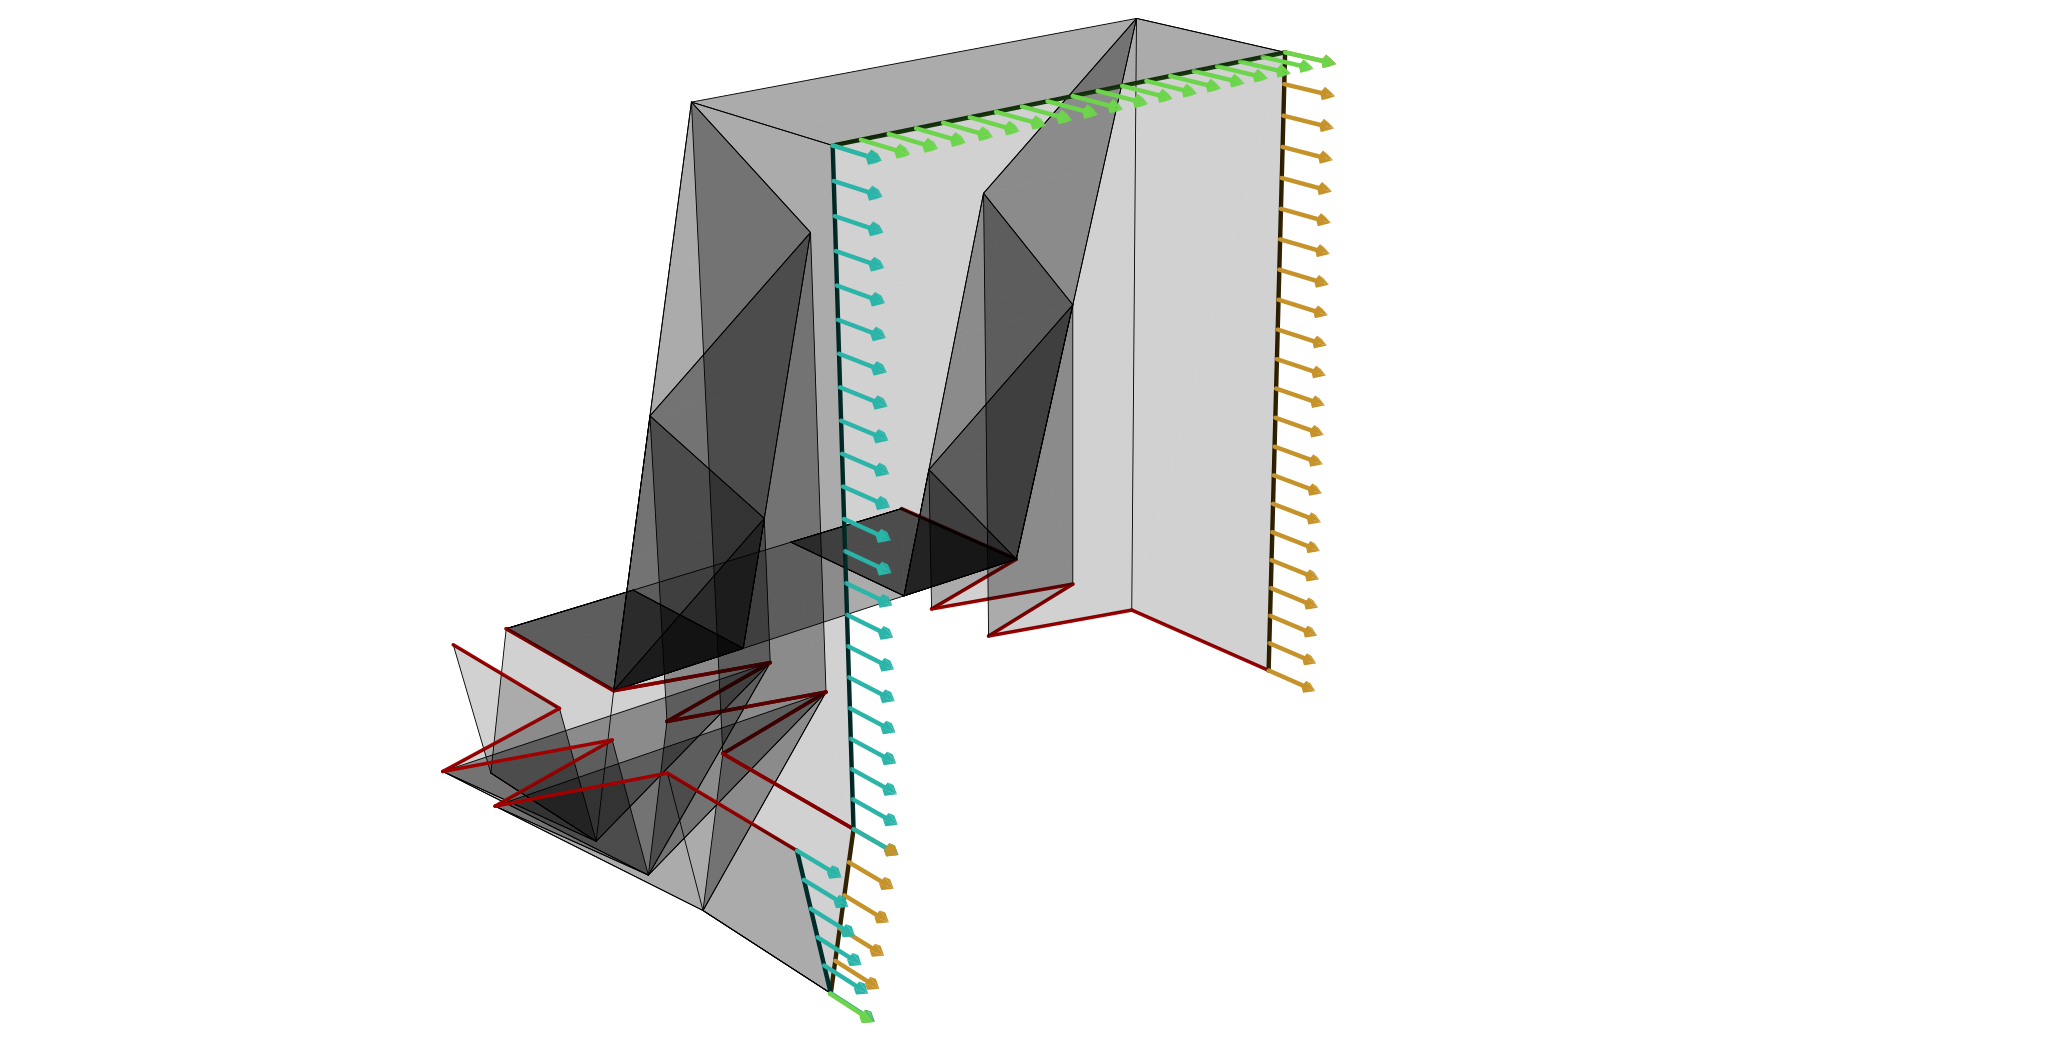
\includegraphics[width=0.34\textwidth]{figures/column_connector/column11.pdf}
    }%

    \subfloat[Connector gadget.]{
        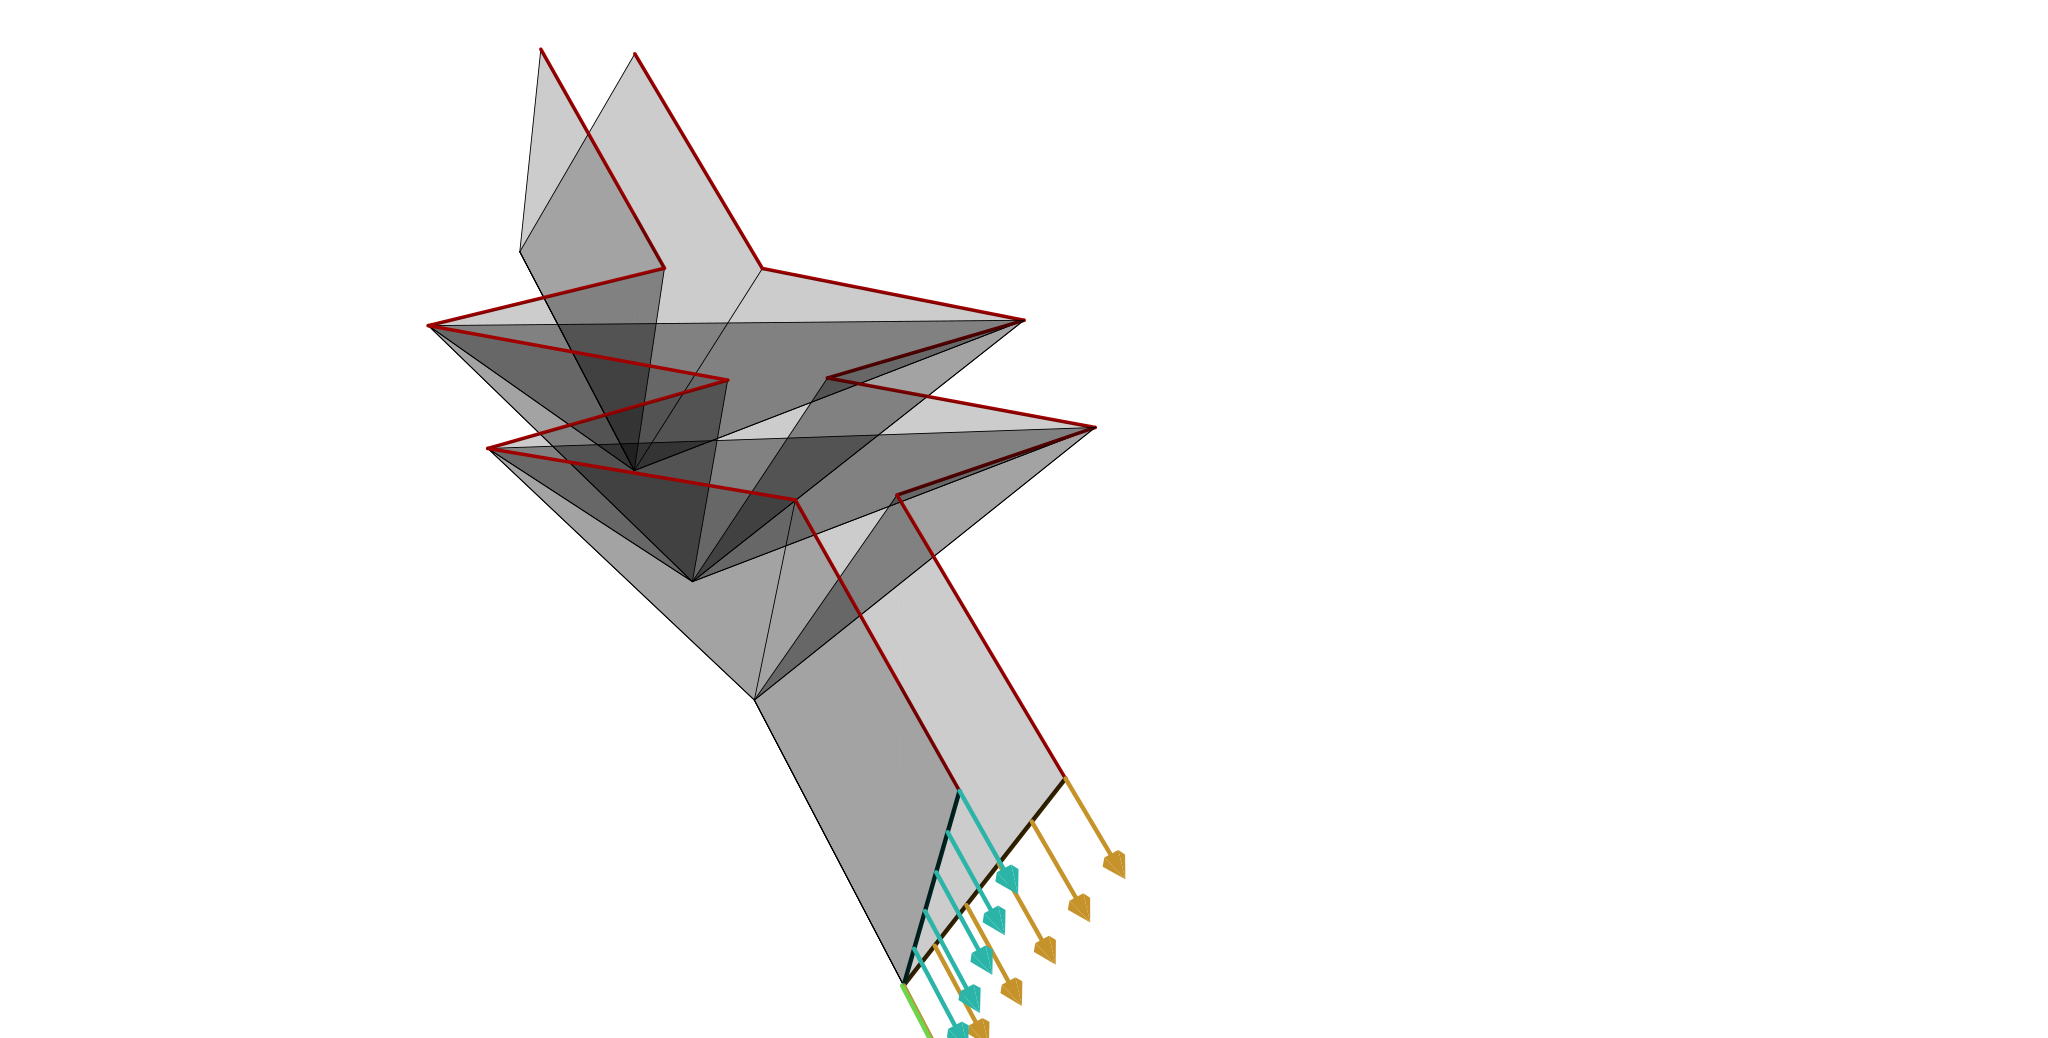
\includegraphics[width=0.31\textwidth]{figures/column_connector/connector0.pdf}
    }%
    \subfloat[Side view.]{
        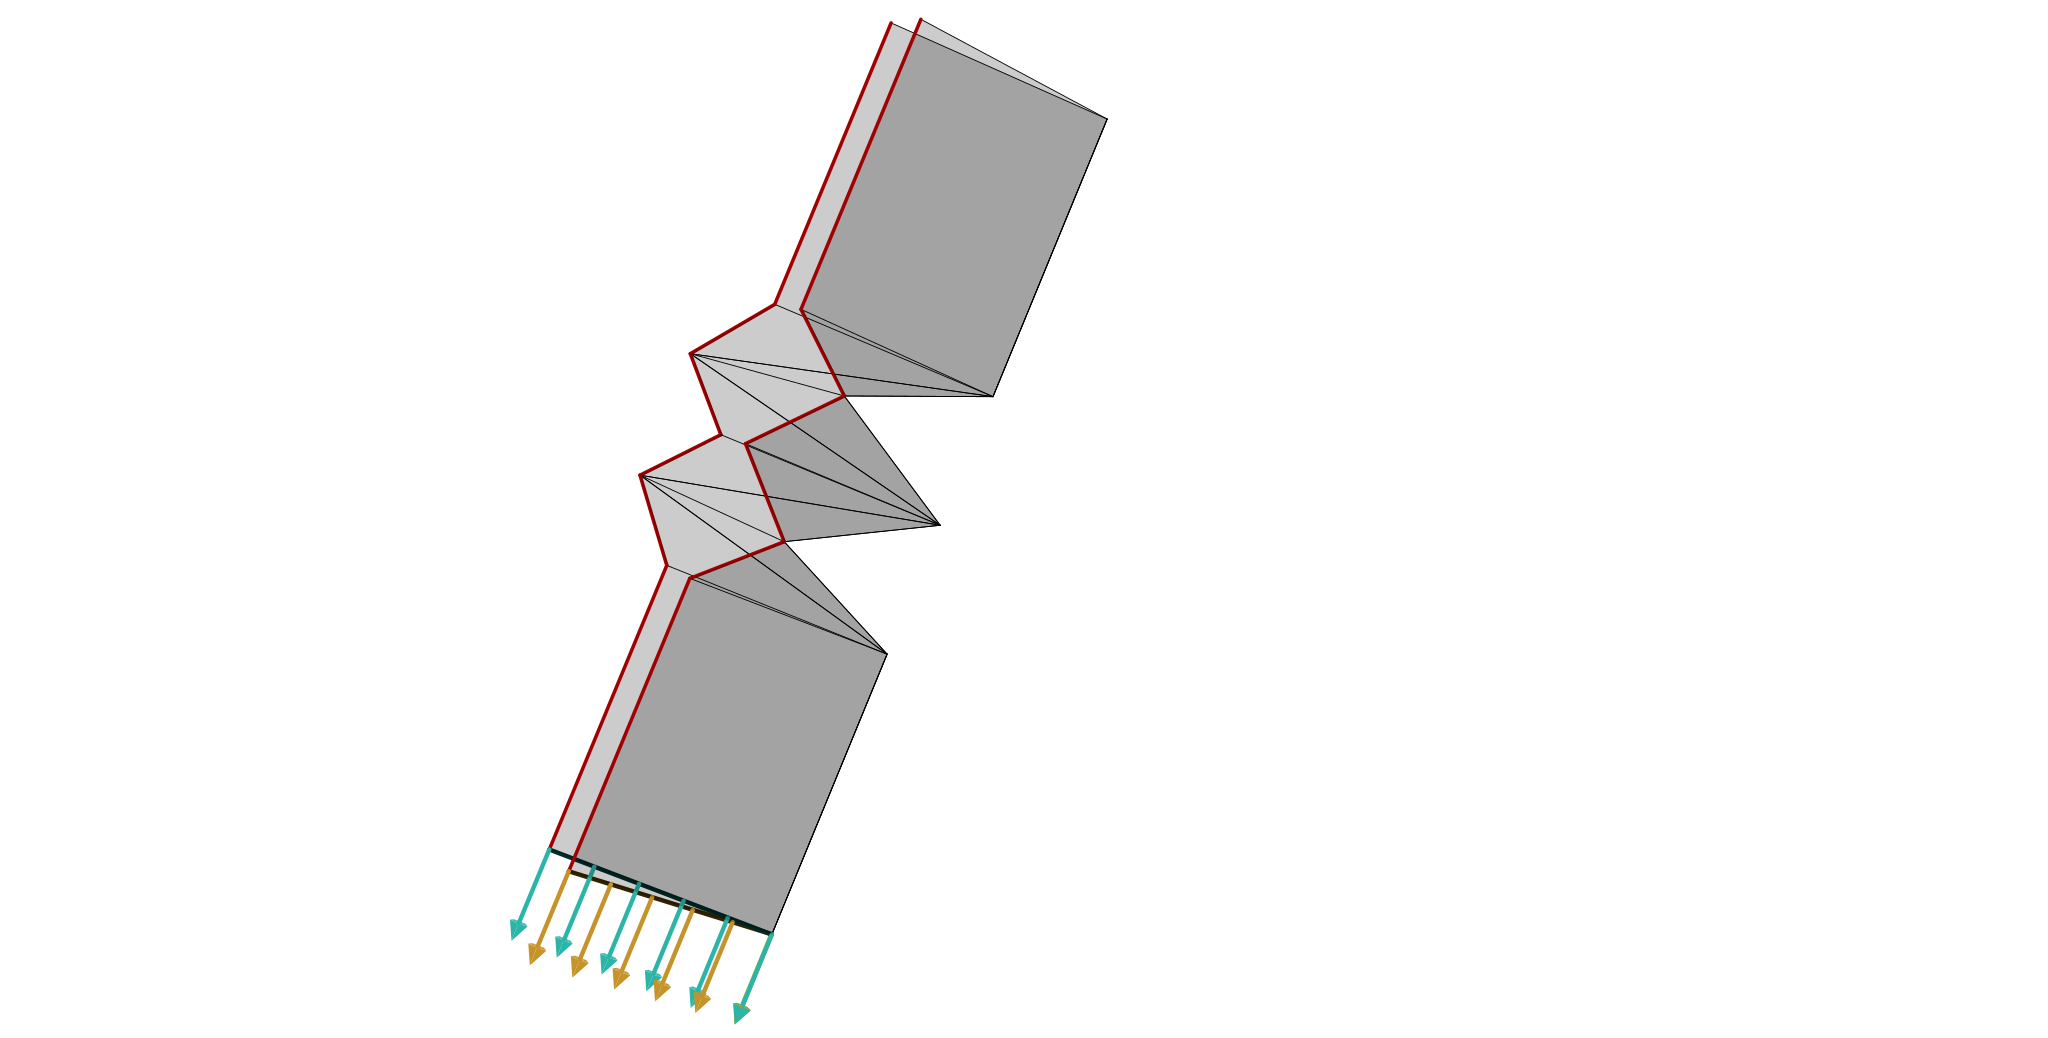
\includegraphics[width=0.27\textwidth]{figures/column_connector/connector1.pdf}
    }%
    \subfloat[Flat folded state.]{
        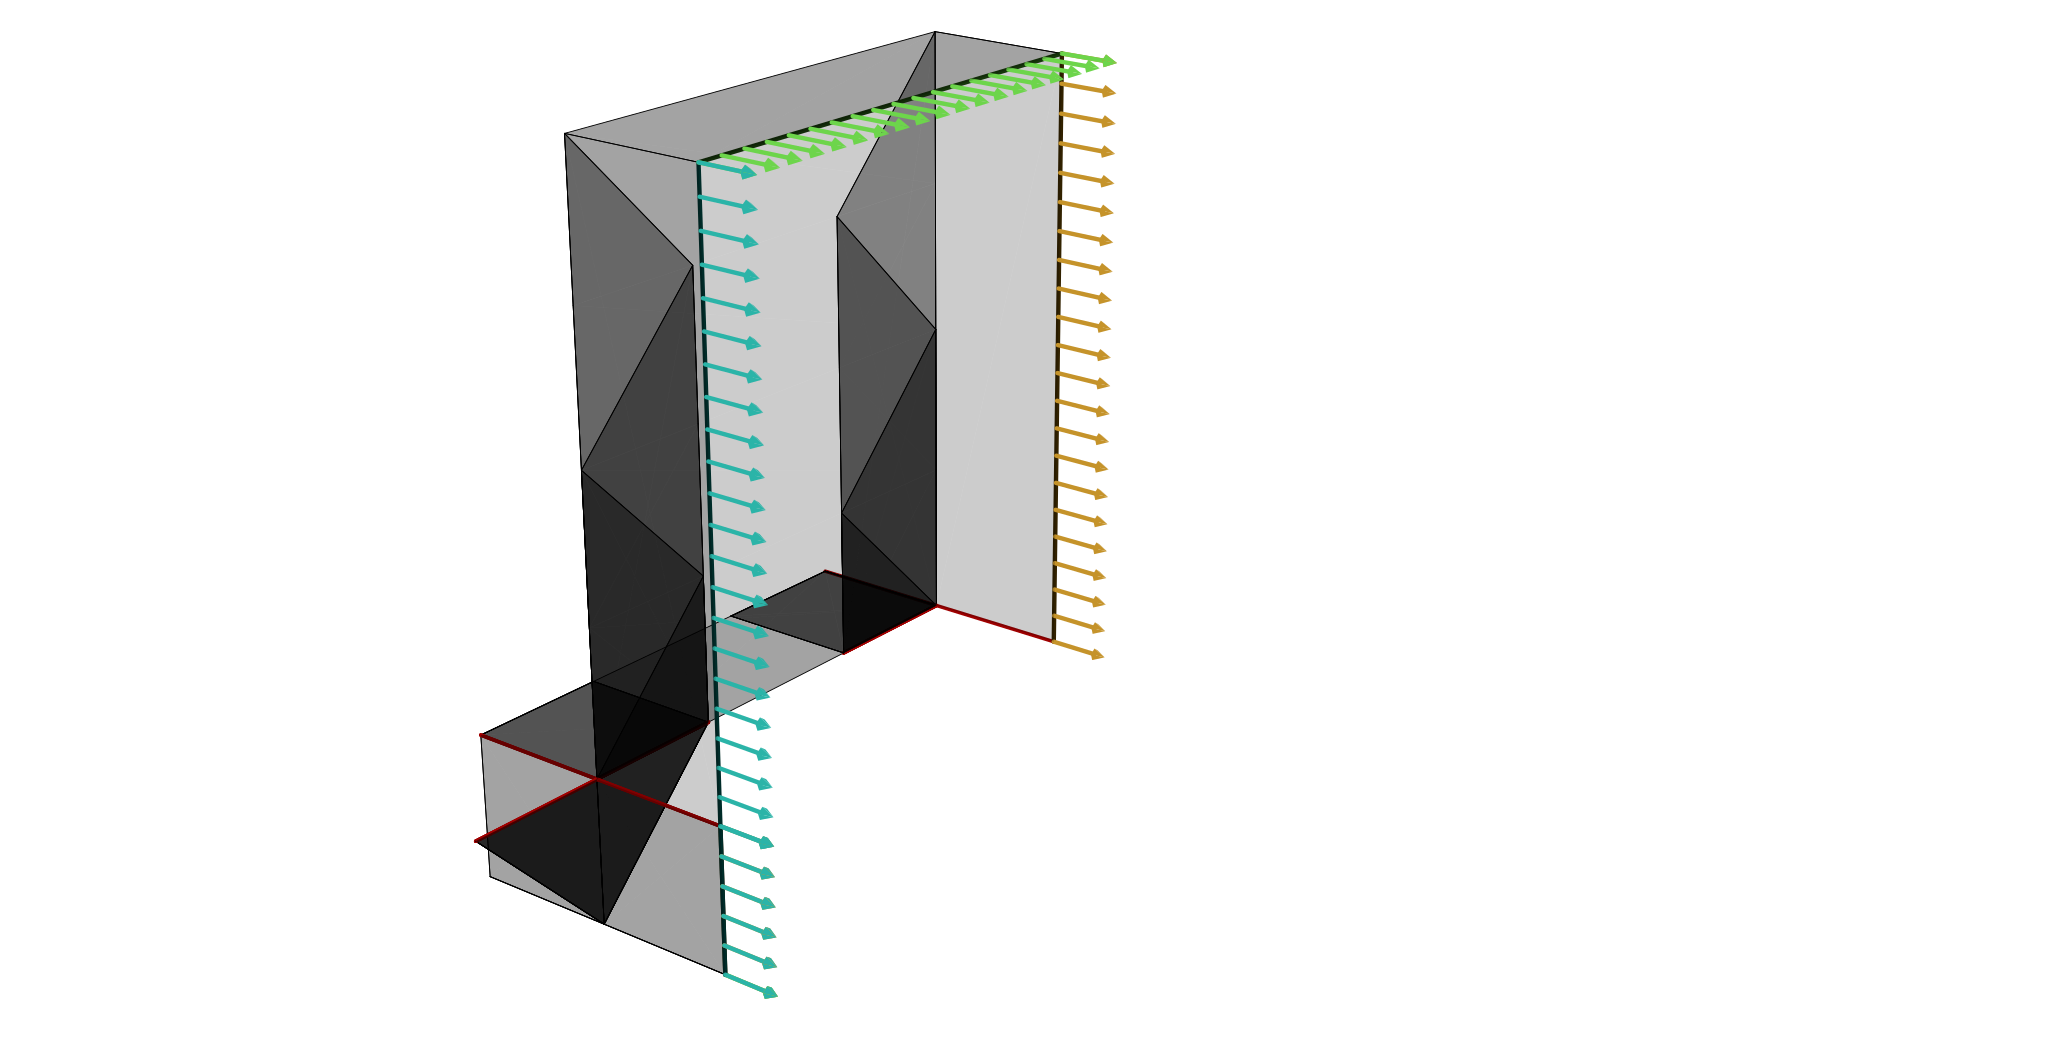
\includegraphics[width=0.31\textwidth]{figures/column_connector/column_connector0.pdf}
    }%
    \caption{
    Column gadget attached to a single column connector gadget.
    The red line demarcates the interface between the two gadgets.
    }
    \label{fig:column_connector}
    \vspace{-20pt}
\end{figure}
\clearpage

